% DSR-Net (DualStreamForensicNet in aigi_jpeg.py) -- editable TikZ source.
% Build: pdflatex architecture.tex  -> architecture.pdf (vector). Designed at \textwidth = 17.46 cm.
\documentclass[tikz,border=1pt]{standalone}
\usepackage{mathptmx}
\usepackage{tikz}
\usetikzlibrary{positioning,arrows.meta,calc,fit,backgrounds,decorations.pathreplacing}

% palette (same hues as the plots): blue = RGB, orange = forensic, grey = trunk, green = head
\definecolor{rgbE}{HTML}{2A78D6}\definecolor{rgbF}{HTML}{E3EEFB}
\definecolor{frE}{HTML}{D2581F}\definecolor{frF}{HTML}{FCE7DC}
\definecolor{trE}{HTML}{6B6A66}\definecolor{trF}{HTML}{EFEEEA}
\definecolor{hdE}{HTML}{15936A}\definecolor{hdF}{HTML}{DDF3EA}
\definecolor{ink}{HTML}{1A1A1A}\definecolor{ink2}{HTML}{5A5955}

\tikzset{
  >={Stealth[length=4pt,width=3.2pt]},
  every node/.style={font=\scriptsize, text=ink, align=center},
  xblk/.style={draw, rounded corners=2pt, line width=0.6pt, inner sep=2.5pt, minimum height=0.95cm, align=center, font=\fontsize{6.2}{7.2}\selectfont},
  xrgb/.style={xblk, draw=rgbE, fill=rgbF},
  xfr/.style={xblk, draw=frE, fill=frF},
  xfrfix/.style={xblk, draw=frE, fill=white, dashed},
  xtr/.style={xblk, draw=trE, fill=trF},
  xhd/.style={xblk, draw=hdE, fill=hdF},
  xio/.style={xblk, draw=ink2, fill=white},
  xflow/.style={->, line width=0.65pt, draw=ink2},
  xdim/.style={font=\fontsize{5.6}{6.4}\selectfont, text=ink2},
  xpar/.style={font=\fontsize{5.6}{6.4}\selectfont\itshape, text=ink2},
  xsub/.style={font=\fontsize{5.8}{6.8}\selectfont},
}
\newcommand{\ttl}[2]{{\scriptsize\bfseries #1}\\[0.5pt]#2}

\begin{document}
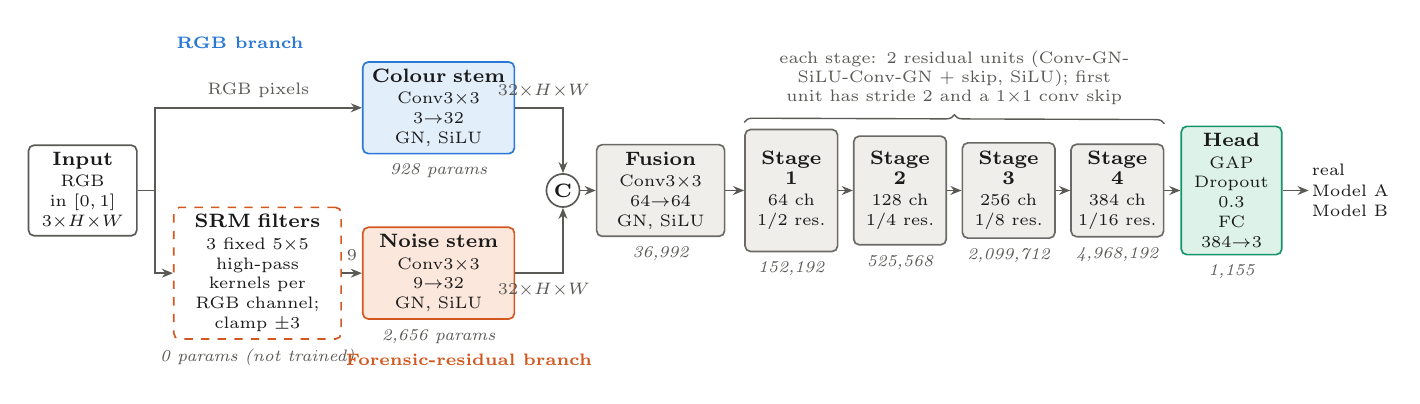
\begin{tikzpicture}
  % ---------------- input ----------------
  \node[xio, text width=1.2cm] (in) at (0.68,0) {\ttl{Input}{RGB in $[0,1]$\\$3{\times}H{\times}W$}};

  % ---------------- two parallel branches ----------------
  \node[xfrfix, text width=1.95cm] (srm) at (2.9,-1.05)
       {\ttl{SRM filters}{3 fixed $5{\times}5$ high-pass kernels per RGB channel; clamp $\pm3$}};
  \node[xfr,  text width=1.75cm] (ns)  at (5.2,-1.05) {\ttl{Noise stem}{Conv$3{\times}3$ 9$\to$32\\GN, SiLU}};
  \node[xrgb, text width=1.75cm] (cs)  at (5.2, 1.05) {\ttl{Colour stem}{Conv$3{\times}3$ 3$\to$32\\GN, SiLU}};

  \draw[xflow] (in.east) -- ++(0.22,0) |- (cs.west) node[pos=0.75, above, xdim] {RGB pixels};
  \draw[xflow] (in.east) -- ++(0.22,0) |- (srm.west);
  \draw[xflow] (srm) -- (ns) node[midway, above=1pt, xdim] {9};

  \node[xpar, below=0pt of cs] {928 params};
  \node[xpar, below=0pt of ns] {2,656 params};
  \node[xpar, below=0pt of srm] {0 params (not trained)};

  \node[font=\fontsize{6.2}{7}\selectfont\bfseries, text=rgbE, anchor=south west] at (1.75,1.68) {RGB branch};
  \node[font=\fontsize{6.2}{7}\selectfont\bfseries, text=frE, anchor=north west] at (3.9,-1.95) {Forensic-residual branch};

  % ---------------- fusion ----------------
  \node[draw=ink2, circle, line width=0.6pt, inner sep=0pt, minimum size=0.42cm, font=\scriptsize\bfseries] (cat) at (6.78,0) {C};
  \draw[xflow] (cs.east) -| (cat.north) node[pos=0.3, above, xdim] {$32{\times}H{\times}W$};
  \draw[xflow] (ns.east) -| (cat.south) node[pos=0.3, below, xdim] {$32{\times}H{\times}W$};
  \node[xtr, text width=1.45cm] (mg) at (8.02,0) {\ttl{Fusion}{Conv$3{\times}3$ 64$\to$64\\GN, SiLU}};
  \draw[xflow] (cat) -- (mg);
  \node[xpar, below=0pt of mg] {36,992};

  % ---------------- trunk: four residual stages ----------------
  \node[xtr, text width=1.0cm, minimum height=1.55cm] (s1) at (9.68,0) {\ttl{Stage 1}{64 ch\\1/2 res.}};
  \node[xtr, text width=1.0cm, minimum height=1.38cm] (s2) at (11.06,0) {\ttl{Stage 2}{128 ch\\1/4 res.}};
  \node[xtr, text width=1.0cm, minimum height=1.21cm] (s3) at (12.44,0) {\ttl{Stage 3}{256 ch\\1/8 res.}};
  \node[xtr, text width=1.0cm, minimum height=1.04cm] (s4) at (13.82,0) {\ttl{Stage 4}{384 ch\\1/16 res.}};
  \draw[xflow] (mg) -- (s1);
  \draw[xflow] (s1) -- (s2); \draw[xflow] (s2) -- (s3); \draw[xflow] (s3) -- (s4);
  \node[xpar, below=0pt of s1] {152,192};
  \node[xpar, below=0pt of s2] {525,568};
  \node[xpar, below=0pt of s3] {2,099,712};
  \node[xpar, below=0pt of s4] {4,968,192};
  \draw[decorate, decoration={brace, amplitude=3pt}, draw=ink2, line width=0.5pt]
       ($(s1.north west)+(0,0.08)$) -- ($(s4.north east)+(0,0.25)$)
       node[midway, above=3pt, xsub, text=ink2, text width=5.2cm]
       {each stage: 2 residual units (Conv-GN-SiLU-Conv-GN $+$ skip, SiLU); first unit has stride 2 and a $1{\times}1$ conv skip};

  % ---------------- classifier head ----------------
  \node[xhd, text width=1.1cm, minimum height=1.25cm] (hd) at (15.27,0) {\ttl{Head}{GAP\\Dropout 0.3\\FC 384$\to$3}};
  \draw[xflow] (s4) -- (hd);
  \node[xpar, below=0pt of hd] {1,155};
  \node[anchor=west, font=\fontsize{6}{7.4}\selectfont, align=left, inner sep=1pt] (out) at (16.25,0) {real\\Model A\\Model B};
  \draw[xflow] (hd.east) -- (out.west);

\end{tikzpicture}
\end{document}
